\scanpage{65}\mspage{64}
Inversement, donnons nous, \deleted{$\unsure{F_i\in|F_i}$} $\unsure{(}\forall i\in I)$ un $F_i\in\mathcal F_i$, quand peut-on dire qu'il existe $F\in\mathcal F$ telle que $\forall i$, $F_i$ soit la $i$ composante de $\deleted{\unsure{\mathcal F}}\unsure{F_0|F}$ ?

Déjà, il le faudrait pour \unsure{le|les} cas où tous les $F_i$ sauf un nb fini sont \deleted{$\varnothing$} vides. On va supposer donc

\uline{$C4$} Si $x,y\in M$ appartiennent à des comp connexes disjointes de $M$, alors $x$ et $y$ sont compatibles.

\deleted{Cor} \inserted{C'est néc et suffisant pour la \unsure{validité|\deleted{val}idité} des}

\uline{Corollaire 1} L'image de $\mathcal F\to\prod\mathcal F_i$ contient les $(F_i)_{i\in I}$ tels que $F_i=\varnothing$ \deleted{sauf} pour \deleted{\unsure{pres}} que tout $i$.

% The added Cor. 2 and its open angular enclosure stand to the right of Corollaire 1's final line.
% The lower-left arm of the enclosure points toward the continuation "est une bijection".
\figure{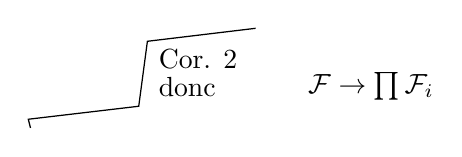
\begin{tikzpicture}[x=0.55cm,y=0.55cm]
\draw[line width=0.45pt] (-2.5,-1.4) -- (-2.55,-1.2) -- (0,-0.9) -- (0.2,0.6) -- (2.7,0.9);
\node[anchor=west,inner sep=0pt] at (0.45,0.2) {\inserted{\uline{Cor. 2}}};
\node[anchor=west,inner sep=0pt] at (0.45,-0.45) {\deleted{\unsure{donc}}};
\node[anchor=west,inner sep=0pt] at (3.9,-0.45) {$\mathcal F\to\prod\mathcal F_i$};
\end{tikzpicture}}
est une bijection dans \unsure{le\deleted{s}|les} \deleted{deux} cas où \deleted{suivants} \inserted{$I$ est fini.}

\deleted{a) $I$ est fini}

\deleted{b) Toute figure est de t.f. -- alors}

\uline{Cor 3} Supposons que les figures \deleted{\unsure{de|des}} $\in\mathcal F$ soient de t.f. \deleted{Alors il} \inserted{(resp. finies)}. Alors il en est de $=$ \deleted{\unsure{de}} pour $\mathcal F_i$, de plus $\mathcal F\unsure{\text{---}|\longrightarrow}\prod\mathcal F_i$ a comme image l'ens des $(F_i)$ tels que $F_i$ soit $\varnothing$ pour \unsure{pres|près|prés} que tout $i$.
